\documentclass[11pt,aspectratio=169]{beamer}

\usepackage[utf8]{inputenc}
\usetheme{Luebeck}
\usepackage[ruled,noline,linesnumbered]{algorithm2e}
\usepackage{minted}
\usepackage{subcaption}
\usepackage{booktabs}

\setbeamertemplate{navigation symbols}{}

\makeatother
\setbeamertemplate{headline}{}
\setbeamertemplate{footline}
{
  \leavevmode%
  \hbox{%
  \begin{beamercolorbox}[wd=.3\paperwidth,ht=2.25ex,dp=1ex,center]{author in head/foot}%
    \usebeamerfont{author in head/foot}\insertshortauthor
  \end{beamercolorbox}%
  \begin{beamercolorbox}[wd=.5\paperwidth,ht=2.25ex,dp=1ex,center]{title in head/foot}%
    \usebeamerfont{title in head/foot}\insertshorttitle\hspace*{3em}
  \end{beamercolorbox}%
  \begin{beamercolorbox}[wd=.2\paperwidth,ht=2.25ex,dp=1ex,right]{title in head/foot}%
    \usebeamerfont{date in head/foot}\insertshortdate{}\hspace*{2em}
    \insertframenumber{} / \inserttotalframenumber\hspace*{2ex}
  \end{beamercolorbox}}%
  \vskip0pt%
}
\makeatletter

\definecolor{UBCblue}{rgb}{0.05, 0.38, 0.64} % UBC Blue (primary)
\definecolor{UBCgrey}{rgb}{0.2, 0.4, 0.6} % UBC Grey (secondary)

\setbeamercolor{palette primary}{bg=UBCblue,fg=white}
\setbeamercolor{palette secondary}{bg=UBCblue,fg=white}
\setbeamercolor{palette tertiary}{bg=UBCblue,fg=white}
\setbeamercolor{palette quaternary}{bg=UBCblue,fg=white}

\setbeamercolor{structure}{fg=UBCblue} % itemize, enumerate, etc
\setbeamercolor{section in toc}{fg=UBCblue} % TOC sections

% Override palette coloring with secondary
\setbeamercolor{subsection in head/foot}{bg=UBCgrey,fg=white}


\newcommand{\etal}{\textit{et al}.}
\newcommand{\ie}{\textit{i}.\textit{e}.}
\newcommand{\eg}{\textit{e}.\textit{g}.}


\title{Regularizing Neural Networks via Adversarial Model Perturbation}
\author[Yaowei Zheng, Richong Zhang, Yongyi Mao]{\textbf{Yaowei Zheng}\inst{1} \and Richong Zhang\inst{1} \and Yongyi Mao\inst{2}}
\institute{
\inst{1}BDBC and SKLSDE, Beihang University, Beijing, China\and
\inst{2}School of EECS, University of Ottawa, Ottawa, Canada
}
\date{CVPR 2021}
\addtobeamertemplate{title page}{\centering
\includegraphics[width=3.5em]{figs/buaa.png}\hspace{1em}
\includegraphics[width=6em]{figs/uottawa.png}}{}

\begin{document}

\frame{\titlepage}

\begin{frame}{Outline}
\tableofcontents
\end{frame}



\section{Background}

% \begin{frame}{Outline}
% \tableofcontents[currentsection]
% \end{frame}

\begin{frame}{Regularization Alleviate Overfitting}

% Regularization is the most important approach in practice to alleviate overfitting and improve generalization. The following figures sketch the generalization behaviour of the deep neural networks.

% Typical regularization techniques improve generalization through various approaches, including:

% However, more {\bf principled} and more {\bf powerful} regularization schemes are yet to be discovered.

Effective regularization schemes alleviate overfitting and improve generalization.

\begin{figure}
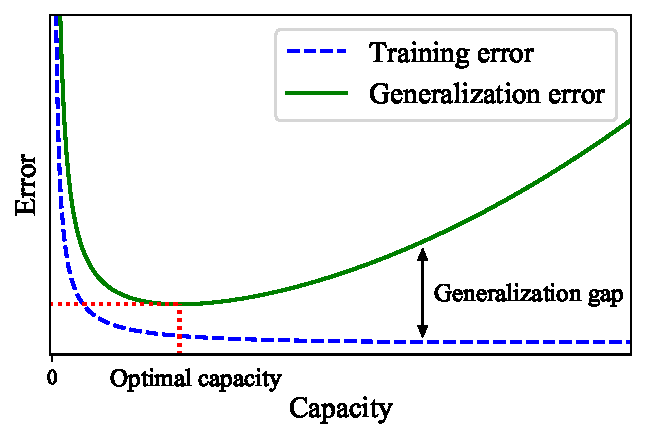
\includegraphics[width=.45\textwidth]{figs/gap1.pdf}
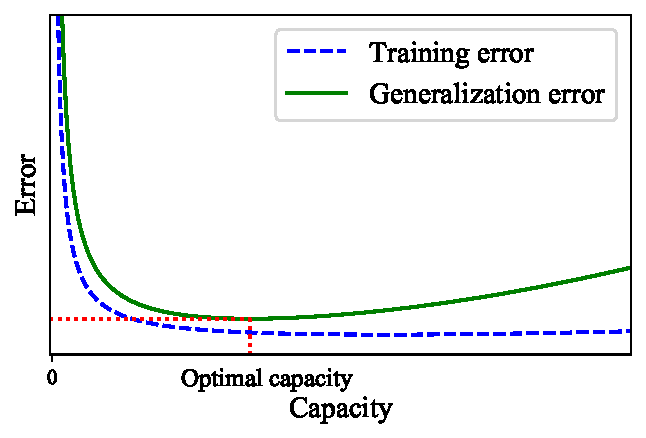
\includegraphics[width=.45\textwidth]{figs/gap2.pdf}
\end{figure}
\vspace{-1em}
{\small
\begin{itemize}
    \item Some researchers have found the modern neural networks may have different behaviour, \ie, the {\em Double Descent} (Nakkiran \etal, 2020). Nevertheless, well-regularized neural networks consistently achieve better performance in practice.
\end{itemize}
}

\end{frame}

\begin{frame}{Flat Minima Helps Generalization}

\begin{itemize}
    \item Flat minima correspond to low-complexity networks. (Hochreiter \etal, 1997)
    \item Small-batch SGD produces flat minima that generalize well. (Keskar \etal, 2017)
    \item Better minimizers of loss function are flatter in visualization. (Li \etal, 2018)
    \item A PAC-Bayes based generalization guarantee for flat minima. (Foret \etal, 2020)
\end{itemize}

\begin{figure}
\subcaptionbox{ResNet without skip connections}[.48\textwidth]{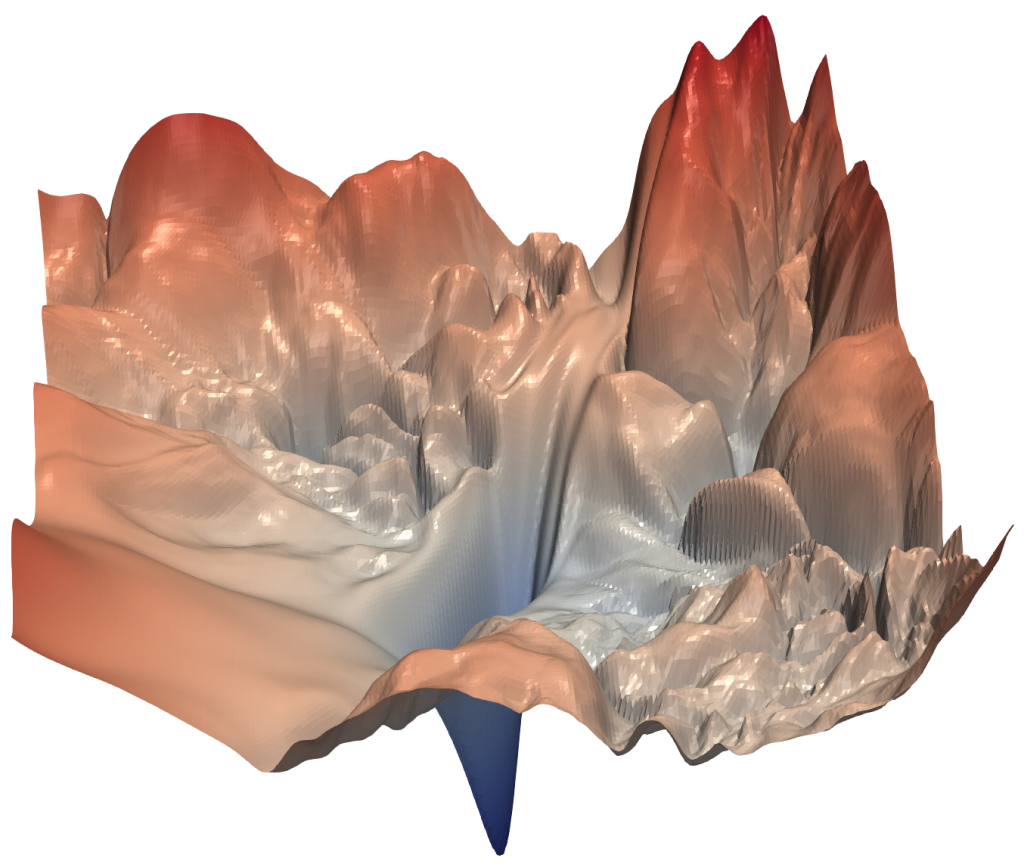
\includegraphics[width=.25\textwidth]{figs/flatness_a.png}}
\subcaptionbox{ResNet with skip connections (Li \etal, 2018)}[.48\textwidth]{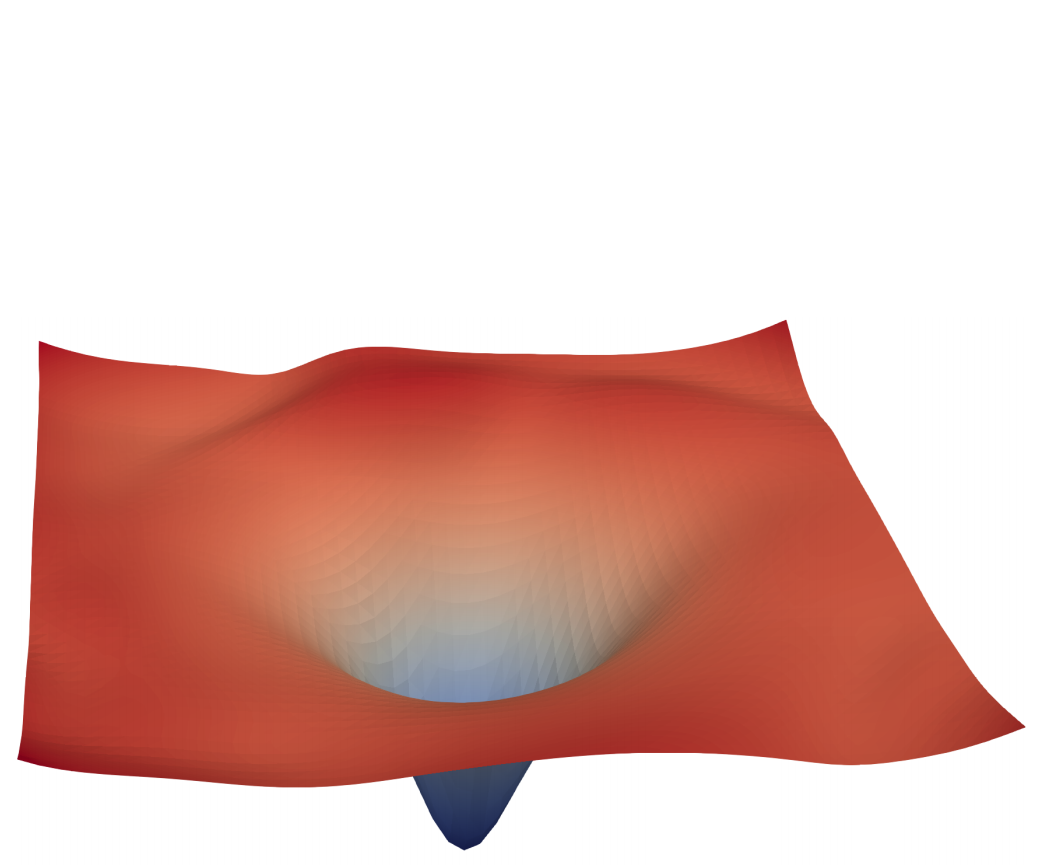
\includegraphics[width=.25\textwidth]{figs/flatness_b.png}}
\end{figure}
\end{frame}

\section{AMP: Adversarial Model Perturbation}

% \begin{frame}{Outline}
% \tableofcontents[currentsection]
% \end{frame}

\begin{frame}{From Empirical Risk to AMP Loss}

\begin{columns}
\column{0.66\textwidth}

The AMP loss is derived from empirical risk by applying the ``worst'' perturbation on the model parameters.

\begin{equation}
\mathcal{L}_\mathrm{ERM}(\boldsymbol{\theta}):=\frac{1}{|D|}\sum_{(\boldsymbol{x},\boldsymbol{y})\in\mathcal{D}}\ell(\boldsymbol{x},\boldsymbol{y};\boldsymbol{\theta})
\end{equation}

\begin{equation}
\mathcal{L}_\mathrm{AMP}(\boldsymbol{\theta}):=\max_{\Delta:\Vert\Delta\Vert\le\epsilon}\mathcal{L}_\mathrm{ERM}(\boldsymbol{\theta}+\Delta)
\end{equation}

As sketched in the figures, it applies a ``max-pooling'' operation on the empirical risk to seek a flatter minima.

\column{0.34\textwidth}
\begin{figure}
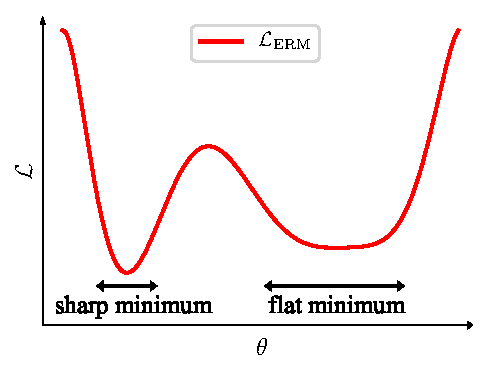
\includegraphics[width=.8\textwidth]{figs/loss_example_a.pdf}
\end{figure}

\begin{figure}
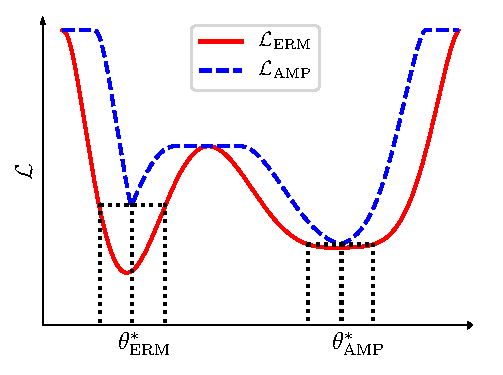
\includegraphics[width=.8\textwidth]{figs/loss_example_b.pdf}
\end{figure}
\end{columns}

\end{frame}


\begin{frame}{Training Algorithm}

A mini-batch SGD is used for solving the ``min-max'' problem.

\begin{equation}
\min_{\boldsymbol{\theta}}\max_{\Delta:\Vert\Delta\Vert\le\epsilon}\mathcal{L}_\mathrm{ERM}(\boldsymbol{\theta}+\Delta)
\end{equation}

\begin{algorithm}[H]
\SetAlgoVlined
\While{$\boldsymbol{\theta}$ not converged}{
Initialize perturbation $\Delta$ with $\boldsymbol{0}$\;
\For{$n\gets1\text{ to }N$}{
Update $\Delta$ to maximize $\!\mathcal{L}_\mathrm{ERM}(\boldsymbol{\theta}\!+\!\Delta)\!$ via gradient ascent with learning rate $\zeta$\;
\If{$\Vert\Delta\Vert_2>\epsilon$}{
Normalize $\Delta$ to restrict its norm $\Vert\Delta\Vert_2$ to $\epsilon$;
}
}
Update $\boldsymbol{\theta}$ to minimize $\mathcal{L}_\mathrm{ERM}(\boldsymbol{\theta}\!+\!\Delta)$ via gradient descent with learning rate $\eta$\;
}
\caption{Adversarial Model Perturbation Training}
\end{algorithm}
\end{frame}

\begin{frame}[fragile]{Implementation}
Source code: \url{https://github.com/hiyouga/AMP-Regularizer}

\begin{minted}[linenos]{python}
from amp import AMP
optimizer = AMP(model.parameters(), lr=0.1, epsilon=0.5, momentum=0.9)
for inputs, targets in dataset:
    def closure():
        optimizer.zero_grad()
        outputs = model(inputs)
        loss = loss_fn(outputs, targets)
        loss.backward()
        return outputs, loss
    outputs, loss = optimizer.step(closure)
\end{minted}
\end{frame}

\section{Theoretical Justifications of AMP}

% \begin{frame}{Outline}
% \tableofcontents[currentsection]
% \end{frame}

\begin{frame}{AMP Finds Flatter Local Minima}

\begin{columns}
\column{0.72\textwidth}

We assume that the loss surface of each local minimum in $\mathcal{L}_\mathrm{ERM}$ can be {\em locally} approximated as an inverted Gaussian surface $\gamma$ with a mean vector $\boldsymbol{\mu}$ and a covariance matrix $\boldsymbol{\kappa}$.
\begin{theorem}[informal]
Under the locally Gaussian assumption, the empirical risk $\gamma(\boldsymbol{\theta};\boldsymbol{\mu},\boldsymbol{\kappa},A,C)$ is minimized when $\boldsymbol{\theta}=\boldsymbol{\mu}$ and the minimum value is $\gamma^\ast(\boldsymbol{\mu},\boldsymbol{\kappa},A,C)=C-A$. The minimum value of the AMP loss is the empirical risk at the location in the narrowest principal direction of the cross-section of the loss surface:
\begin{equation}
\gamma_\mathrm{AMP}^\ast(\boldsymbol{\mu},\boldsymbol{\kappa},A,C)=C-A\exp\left(-\frac{\epsilon^2}{2\sigma^2}\right)
\end{equation}
where $\sigma^2$ is the smallest eigenvalue of $\boldsymbol{\kappa}$.
\end{theorem}

% It is clear that $\gamma^\ast_\mathrm{AMP}$ although related to the minimum value of empirical risk $\gamma^\ast$, it also takes into account the curvature of the surface around the local minimum. Thus we can find a flatter minimum through minimizing $\mathcal{L}_\mathrm{AMP}$.

\column{0.28\textwidth}
\begin{figure}
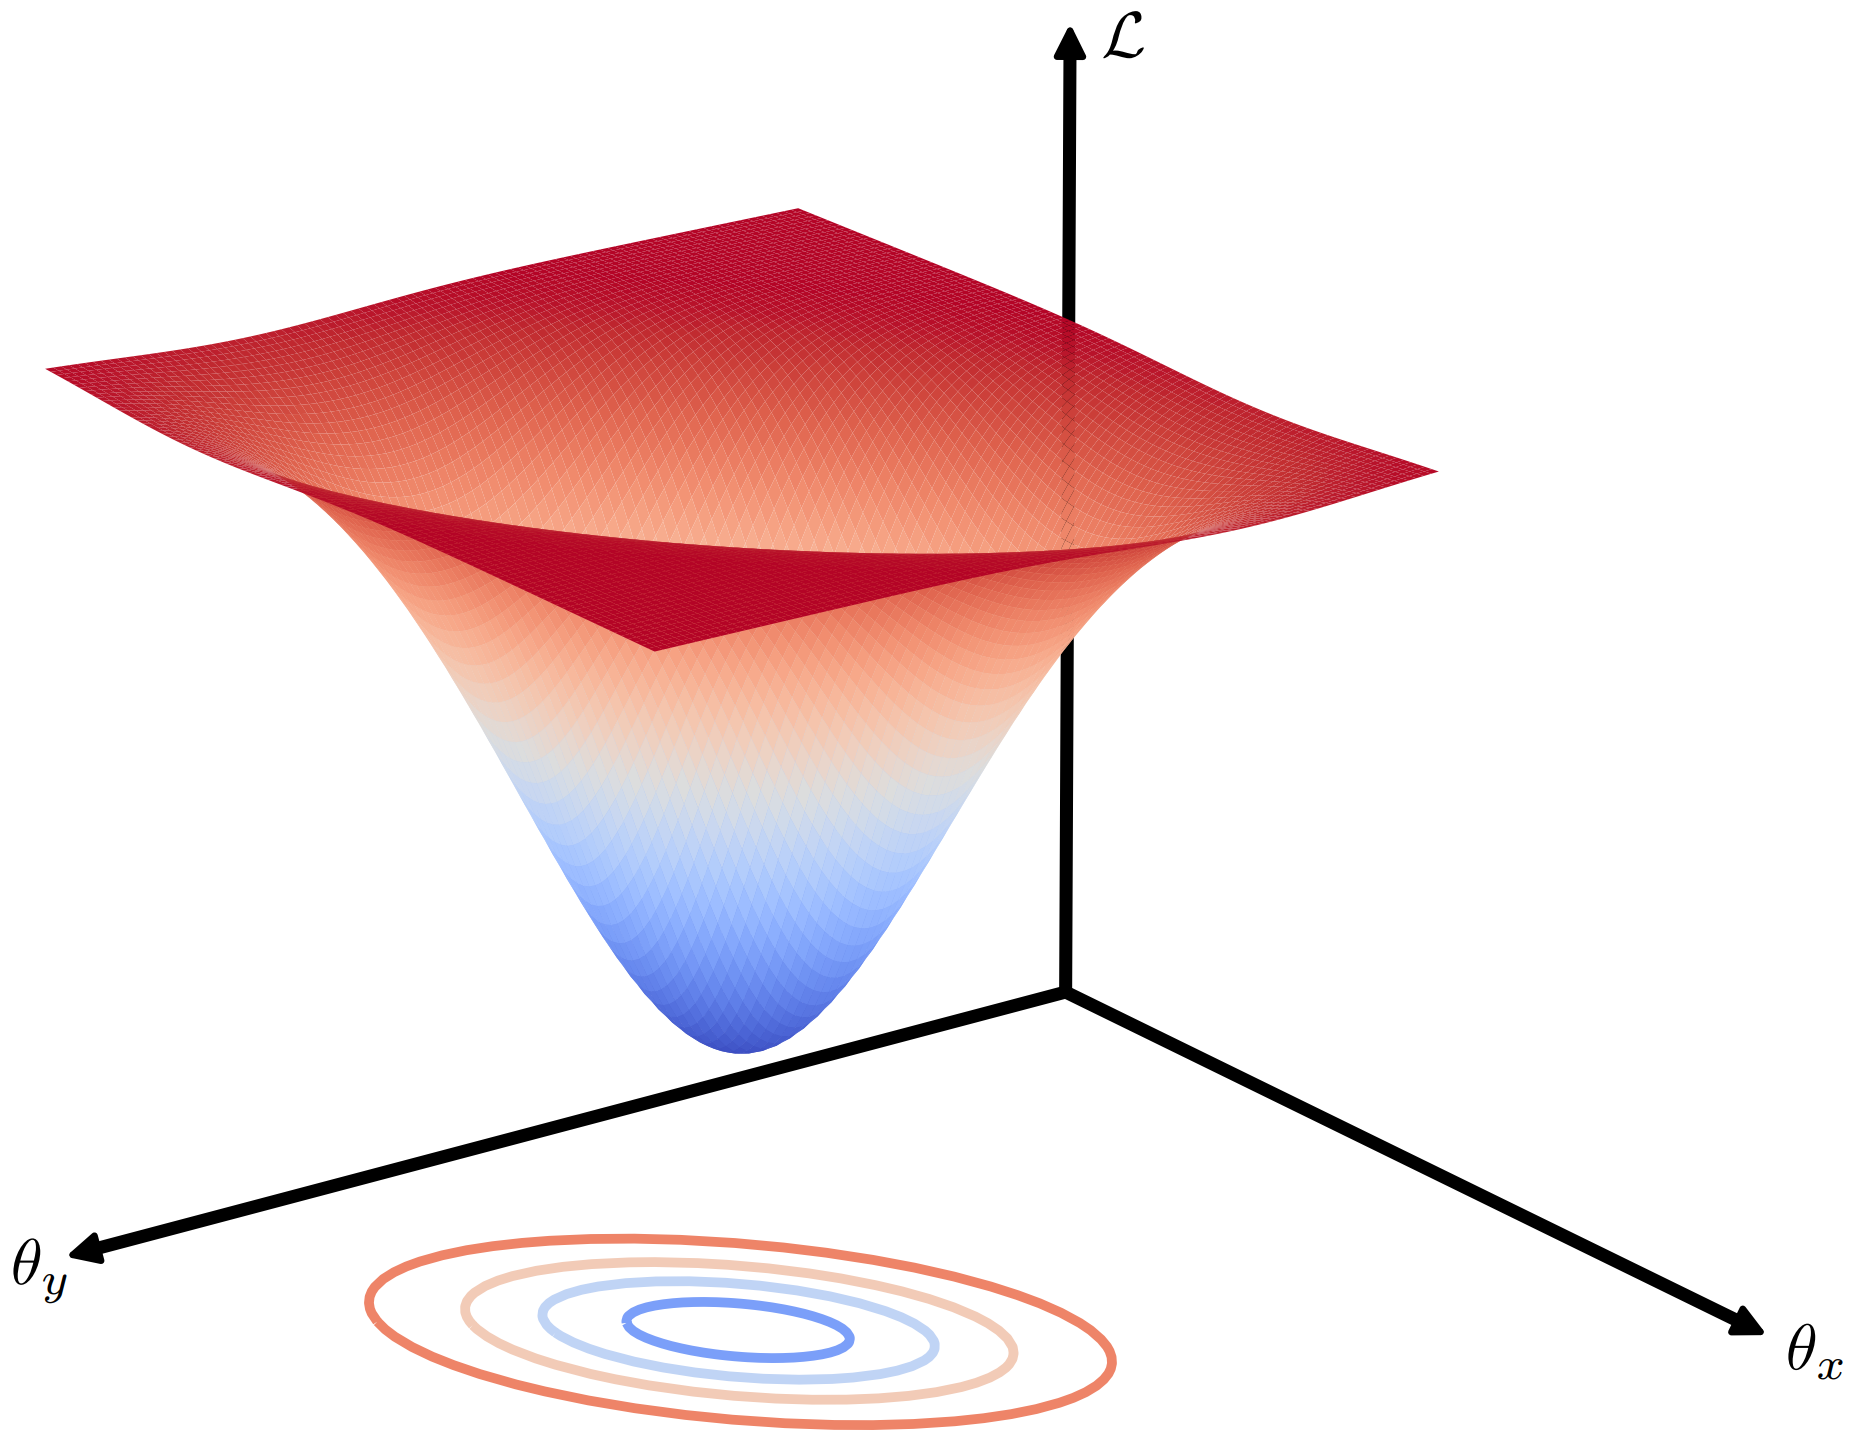
\includegraphics[width=.8\textwidth]{figs/surface.png}
\end{figure}
\begin{figure}
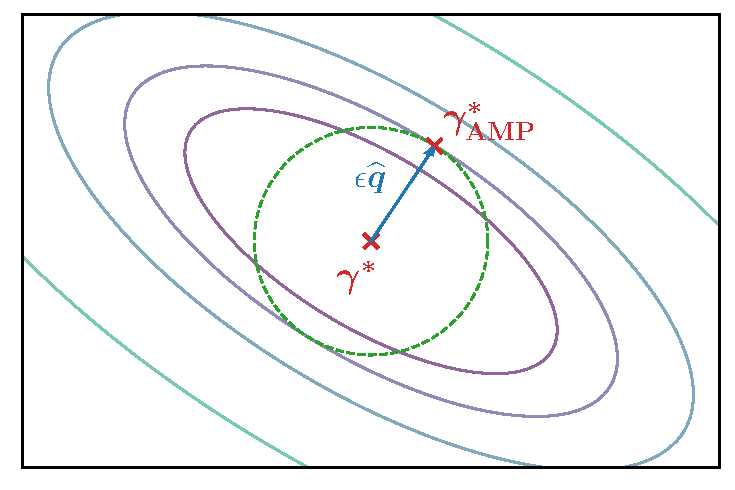
\includegraphics[width=.8\textwidth]{figs/gaussian.pdf}
\caption{The minimum values of $\gamma$ and $\gamma_\mathrm{AMP}$.}
\end{figure}
\end{columns}

\end{frame}

\begin{frame}{AMP Regularizes Gradient Norm}

\begin{theorem}[informal]
Consider that $N=1$, which is in fact used in our experiments. The AMP training is equivalent to ERM training with an additional term:
\begin{equation}
\widetilde{\mathcal{J}}_\mathrm{ERM}(\boldsymbol{\theta}):=\mathcal{J}_\mathrm{ERM}(\boldsymbol{\theta})+\Omega(\boldsymbol{\theta})
\end{equation}
where
\begin{equation}
\Omega(\boldsymbol{\theta}):=\begin{cases}
\zeta\Vert\nabla_{\boldsymbol{\theta}}\mathcal{J}_\mathrm{ERM}(\boldsymbol{\theta})\Vert_2^2,&\Vert\zeta\nabla_{\boldsymbol{\theta}}\mathcal{J}_\mathrm{ERM}(\boldsymbol{\theta})\Vert_2\le\epsilon\\
\epsilon\Vert\nabla_{\boldsymbol{\theta}}\mathcal{J}_\mathrm{ERM}(\boldsymbol{\theta})\Vert_2,&\Vert\zeta\nabla_{\boldsymbol{\theta}}\mathcal{J}_\mathrm{ERM}(\boldsymbol{\theta})\Vert_2>\epsilon
\end{cases}
\end{equation}
\end{theorem}

% Thus, the AMP training algorithm effectively tries to find the local minima of empirical risk that not only have low values, but also have small gradient norm near the minima. Note that a minimum with smaller gradient norms around it is a flatter minimum.

\end{frame}

\section{Experiments}

% \begin{frame}{Outline}
% \tableofcontents[currentsection]
% \end{frame}

\begin{frame}{Experimental Setup}

\begin{columns}
\column{0.4\textwidth}
Image classification datasets:
\begin{itemize}
    \item SVHN (10-way)
    \item CIFAR-10 (10-way)
    \item CIFAR-100 (100-way)
\end{itemize}

\column{0.6\textwidth}

Model architectures:
\begin{itemize}
    \item PreActResNet18 (He \etal, 2016)
    \item VGG16 (Simonyan \etal, 2015)
    \item WideResNet-28-10 (Zagoruyko \etal, 2016)
    \item PyramidNet-164-270 (Han \etal, 2017)
\end{itemize}
\end{columns}

\begin{columns}
\column{0.7\textwidth}
Compared methods:
\begin{itemize}
    \item ERM (Vapnik \etal, 1998)
    \item Dropout (Srivastava \etal, 2014)
    \item Label smoothing (Szegedy \etal, 2016)
    \item Flooding (Ishida \etal, 2020)
    \item MixUp (Zhang \etal, 2018)
    \item Adversarial Training (Goodfellow \etal, 2015)
\end{itemize}
\column{0.3\textwidth}
\end{columns}

\vspace{1.5em}

\end{frame}


\begin{frame}{Loss Curves}

\begin{figure}
\subcaptionbox{CIFAR-10 Training Set}[.48\textwidth]{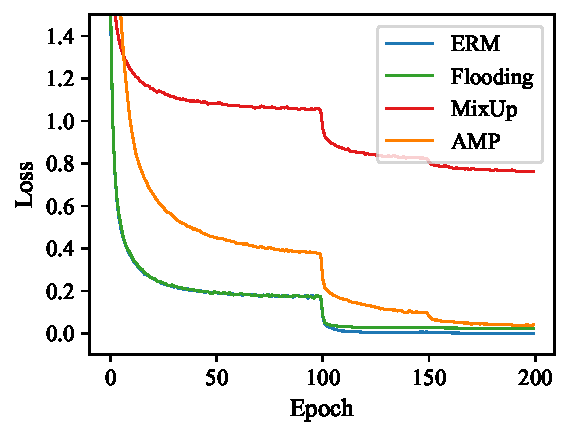
\includegraphics[width=.45\textwidth]{figs/cifar10_preactresnet18_train_loss.pdf}}
\subcaptionbox{CIFAR-10 Test Set}[.48\textwidth]{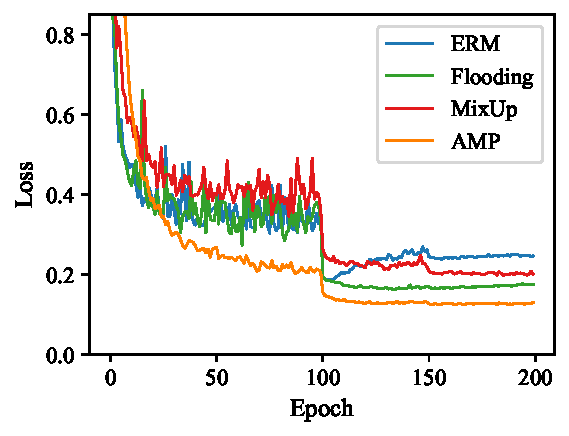
\includegraphics[width=.45\textwidth]{figs/cifar10_preactresnet18_test_loss.pdf}}
\end{figure}

\end{frame}

\begin{frame}{Results on Image Classification Benchmarks}

\begin{table}[t]
\centering
\subcaptionbox{SVHN\label{tab:svhn}}[.33\textwidth]{%
\resizebox{.33\textwidth}{!}{%
\begin{tabular}{lcc}
\toprule
PreActResNet18 & Test Error (\%) & Test NLL \\
\midrule
ERM & 2.95$\pm$0.063 & 0.166$\pm$0.004 \\
Dropout & 2.80$\pm$0.065 & 0.156$\pm$0.012 \\
Label Smoothing & 2.78$\pm$0.087 & 0.998$\pm$0.002 \\
Flooding & 2.84$\pm$0.047 & \underline{0.130$\pm$0.003} \\
MixUp & \underline{2.74$\pm$0.044} & 0.146$\pm$0.004 \\
Adv. Training & 2.77$\pm$0.080 & 0.151$\pm$0.018 \\
RMP & 2.93$\pm$0.066 & 0.161$\pm$0.010 \\
AMP & \textbf{2.30$\pm$0.025} & \textbf{0.096$\pm$0.002} \\
\midrule
VGG16 & Test Error (\%) & Test NLL \\
\midrule
ERM & 3.14$\pm$0.060 & 0.140$\pm$0.027 \\
Dropout & 2.96$\pm$0.049 & 0.134$\pm$0.027 \\
Label Smoothing & 3.07$\pm$0.070 & 1.004$\pm$0.002 \\
Flooding & 3.15$\pm$0.085 & 0.128$\pm$0.003 \\
MixUp & 3.09$\pm$0.057 & 0.160$\pm$0.003 \\
Adv. Training & \underline{2.94$\pm$0.091} & \underline{0.122$\pm$0.003} \\
RMP & 3.19$\pm$0.052 & 0.134$\pm$0.004 \\
AMP & \textbf{2.73$\pm$0.015} & \textbf{0.116$\pm$0.006} \\
\bottomrule
\end{tabular}
}%
}%
\subcaptionbox{CIFAR-10\label{tab:cifar10}}[.33\textwidth]{%
\resizebox{.33\textwidth}{!}{%
\begin{tabular}{lcc}
\toprule
PreActResNet18 & Test Error (\%) & Test NLL \\
\midrule
ERM & 5.02$\pm$0.212 & 0.239$\pm$0.009 \\
Dropout & 4.86$\pm$0.148 & 0.223$\pm$0.009 \\
Label Smoothing & 4.85$\pm$0.115 & 1.038$\pm$0.003 \\
Flooding & 4.97$\pm$0.082 & \underline{0.166$\pm$0.003} \\
MixUp & \underline{4.09$\pm$0.117} & 0.198$\pm$0.004 \\
Adv. Training & 4.99$\pm$0.085 & 0.247$\pm$0.006 \\
RMP & 4.97$\pm$0.167 & 0.239$\pm$0.008 \\
AMP & \textbf{3.97$\pm$0.091} & \textbf{0.129$\pm$0.003} \\
\midrule
VGG16 & Test Error (\%) & Test NLL \\
\midrule
ERM & 6.32$\pm$0.193 & 0.361$\pm$0.012 \\
Dropout & 6.22$\pm$0.147 & 0.314$\pm$0.009 \\
Label Smoothing & 6.29$\pm$0.158 & 1.076$\pm$0.003 \\
Flooding & 6.26$\pm$0.145 & \underline{0.234$\pm$0.005} \\
MixUp & \textbf{5.48$\pm$0.112} & 0.251$\pm$0.003 \\
Adv. Training & 6.49$\pm$0.130 & 0.380$\pm$0.010 \\
RMP & 6.30$\pm$0.109 & 0.363$\pm$0.010 \\
AMP & \underline{5.65$\pm$0.147} & \textbf{0.207$\pm$0.005} \\
\bottomrule
\end{tabular}
}%
}%
\subcaptionbox{CIFAR-100\label{tab:cifar100}}[.33\textwidth]{%
\resizebox{.33\textwidth}{!}{%
\begin{tabular}{lcc}
\toprule
PreActResNet18 & Test Error (\%) & Test NLL \\
\midrule
ERM & 24.31$\pm$0.303 & 1.056$\pm$0.013 \\
Dropout & 24.48$\pm$0.351 & 1.110$\pm$0.021 \\
Label Smoothing & 22.07$\pm$0.256 & 2.099$\pm$0.005 \\
Flooding & 24.50$\pm$0.234 & 0.950$\pm$0.011 \\
MixUp & \underline{21.78$\pm$0.210} & \underline{0.910$\pm$0.007} \\
Adv. Training & 25.23$\pm$0.229 & 1.110$\pm$0.012 \\
RMP & 24.28$\pm$0.138 & 1.059$\pm$0.011 \\
AMP & \textbf{21.51$\pm$0.308} & \textbf{0.774$\pm$0.016} \\
\midrule
VGG16 & Test Error (\%) & Test NLL \\
\midrule
ERM & 27.84$\pm$0.297 & 1.827$\pm$0.209 \\
Dropout & 27.72$\pm$0.337 & 1.605$\pm$0.062 \\
Label Smoothing & 27.49$\pm$0.179 & 2.310$\pm$0.005 \\
Flooding & 27.93$\pm$0.271 & 1.221$\pm$0.037 \\
MixUp & \underline{26.81$\pm$0.254} & \underline{1.136$\pm$0.013} \\
Adv. Training & 29.12$\pm$0.145 & 1.535$\pm$0.389 \\
RMP & 27.81$\pm$0.327 & 1.873$\pm$0.035 \\
AMP & \textbf{25.60$\pm$0.168} & \textbf{1.049$\pm$0.049} \\
\bottomrule
\end{tabular}
}%
}%
\caption{Top-1 classification errors and test neg-log-likelihoods.}
\end{table}

\end{frame}

\begin{frame}{Improvement over Data Augmentation}

\begin{table}[t]
\centering
\resizebox{.9\columnwidth}{!}{%
\begin{tabular}{llcccc}
\toprule
 & & \multicolumn{2}{c}{WideResNet-28-10} & \multicolumn{2}{c}{PyramidNet-164-270}\\
 & & ERM & AMP & ERM & AMP \\
\midrule
 & Vanilla & 2.57$\pm$0.067 & \textbf{2.19$\pm$0.036} & 2.47$\pm$0.034 & \textbf{2.11$\pm$0.041} \\
SVHN & Cutout & 2.27$\pm$0.085 & \textbf{1.83$\pm$0.018} & 2.19$\pm$0.021 & \textbf{1.82$\pm$0.023} \\
 & AutoAug & 1.91$\pm$0.059 & \textbf{1.61$\pm$0.024} & 1.80$\pm$0.044 & \textbf{1.35$\pm$0.056} \\
\midrule
 & Vanilla & 3.87$\pm$0.167 & \textbf{3.00$\pm$0.059} & 3.60$\pm$0.197 & \textbf{2.75$\pm$0.040} \\
CIFAR-10 & Cutout & 3.38$\pm$0.081 & \textbf{2.67$\pm$0.043} & 2.83$\pm$0.102 & \textbf{2.27$\pm$0.034} \\
 & AutoAug & 2.78$\pm$0.134 & \textbf{2.32$\pm$0.097} & 2.49$\pm$0.128 & \textbf{1.98$\pm$0.062} \\
\midrule
 & Vanilla & 19.17$\pm$0.270 & \textbf{17.33$\pm$0.110} & 17.13$\pm$0.210 & \textbf{15.09$\pm$0.092} \\
CIFAR-100 & Cutout & 18.12$\pm$0.114 & \textbf{16.04$\pm$0.071} & 16.45$\pm$0.136 & \textbf{14.34$\pm$0.153} \\
 & AutoAug & 17.79$\pm$0.185 & \textbf{14.95$\pm$0.088} & 15.43$\pm$0.269 & \textbf{13.36$\pm$0.245} \\
\bottomrule
\end{tabular}
}
\caption{Top-1 classification errors and test neg-log-likelihoods.}
\end{table}

\end{frame}

\begin{frame}{Calibration Results}

Expected Calibration Error: (lower is better)
\begin{equation*}
\text{ECE}=\sum_{m=1}^M\frac{|B_m|}{n}\bigg\vert\underbrace{\frac{1}{|B_m|}\sum_{i\in B_m}\mathbf{1}(\hat{y}_i=y_i)}_{\text{accuracy}}-\underbrace{\frac{1}{|B_m|}\sum_{i\in B_m}\hat{p}_i}_{\text{confidence}}\bigg\vert
\end{equation*}
\vspace{-0.5em}

\begin{figure}
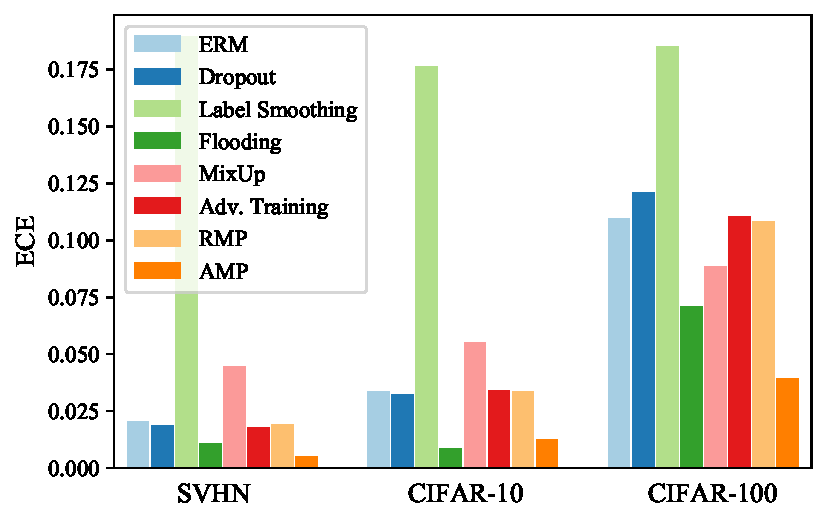
\includegraphics[width=.46\textwidth]{figs/ece.pdf}
\end{figure}

\vspace{1em}

\end{frame}

\begin{frame}{Loss Values with Varying Perturbation Size}

\begin{figure}
\subcaptionbox{CIFAR-10 Training Set}[.48\textwidth]{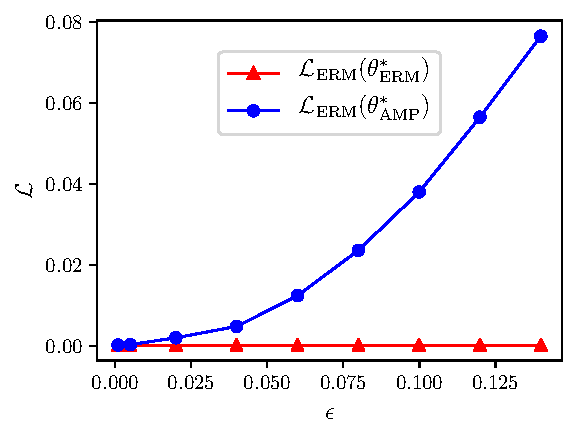
\includegraphics[width=.45\textwidth]{figs/tune_a.pdf}}
\subcaptionbox{CIFAR-10 Test Set}[.48\textwidth]{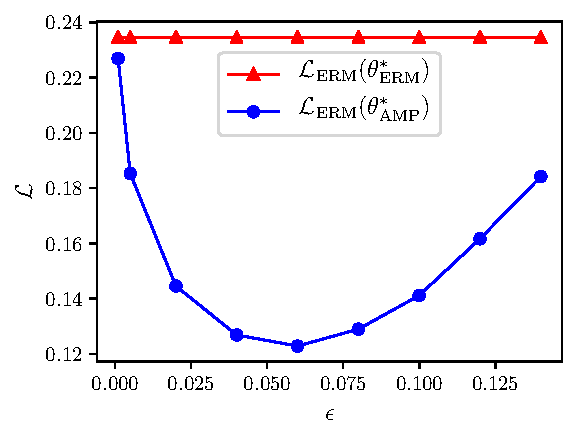
\includegraphics[width=.45\textwidth]{figs/tune_b.pdf}}
\end{figure}

\end{frame}

\begin{frame}{Flatness of the Selected Minima}
\begin{figure}
\subcaptionbox{ERM Training Loss}[.48\textwidth]{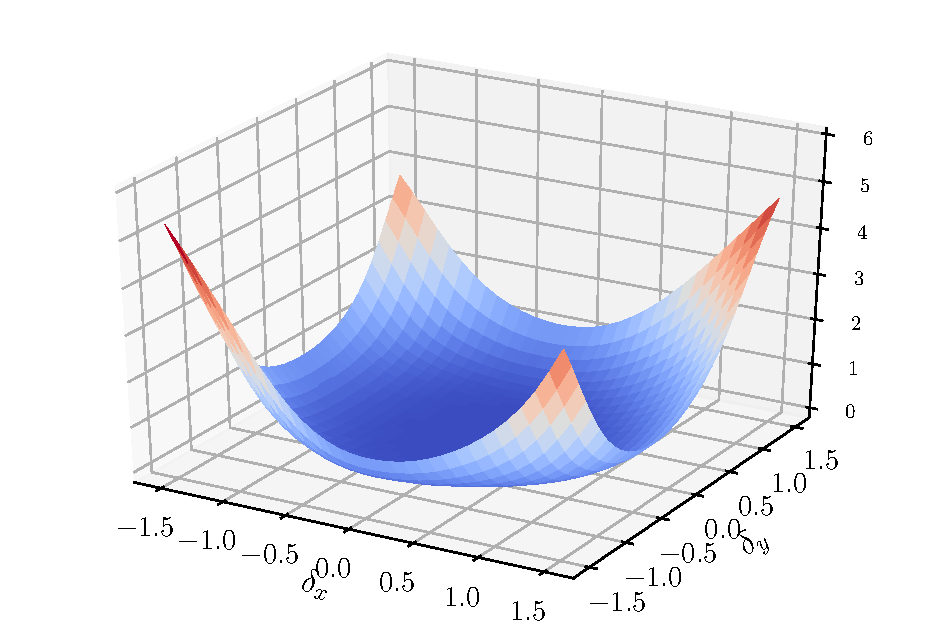
\includegraphics[width=.28\textwidth]{figs/svhn_erm_train_loss_landscape3D.pdf}}
\subcaptionbox{ERM Test Loss}[.48\textwidth]{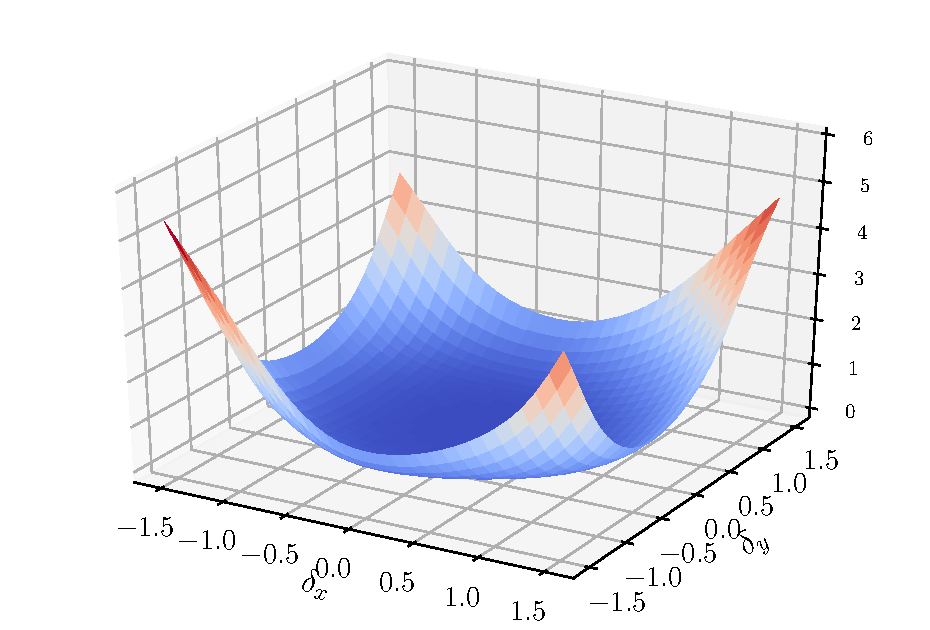
\includegraphics[width=.28\textwidth]{figs/svhn_erm_test_loss_landscape3D.pdf}}
\subcaptionbox{AMP Training Loss}[.48\textwidth]{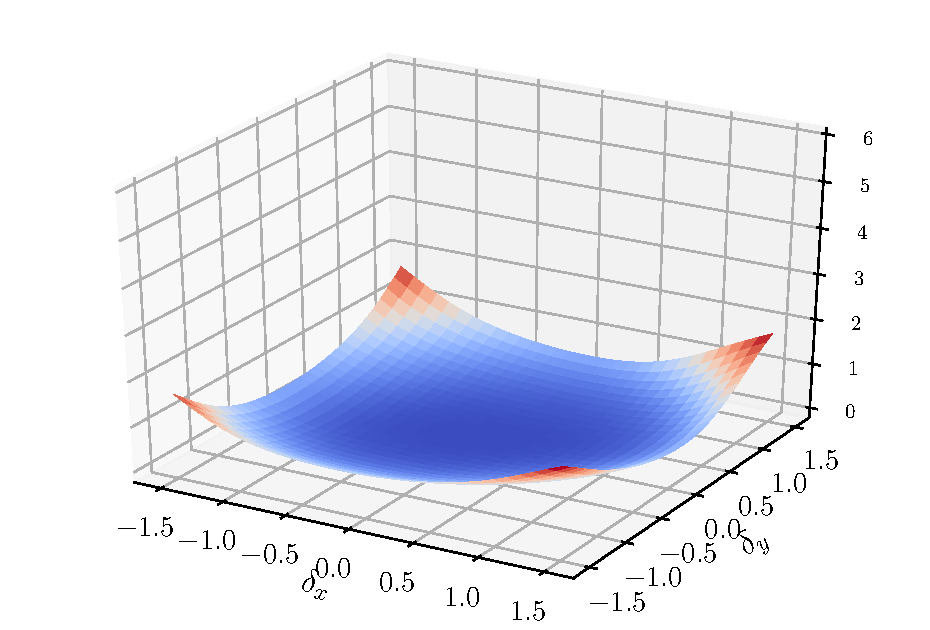
\includegraphics[width=.28\textwidth]{figs/svhn_amp_train_loss_landscape3D.pdf}}
\subcaptionbox{AMP Test Loss}[.48\textwidth]{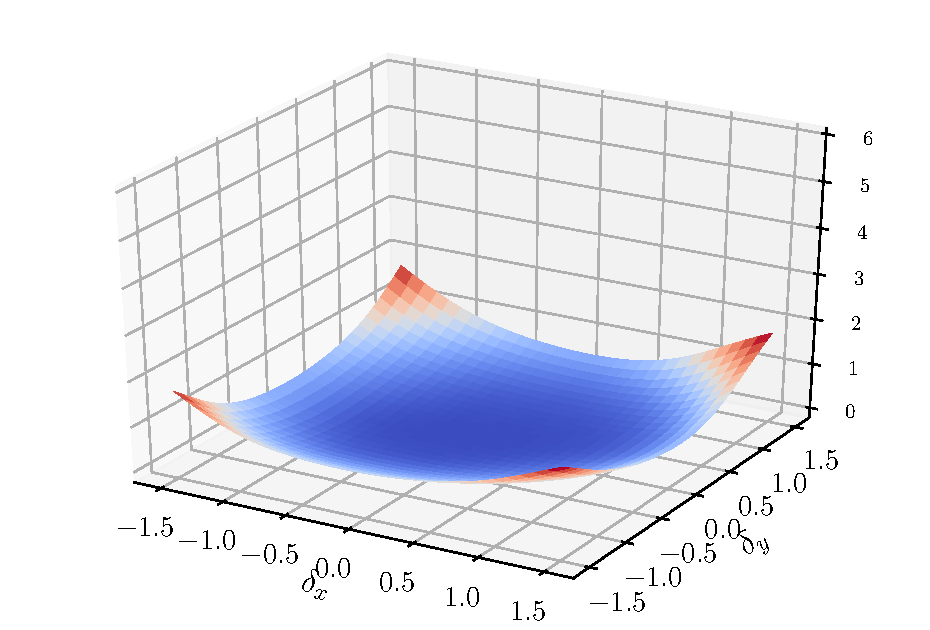
\includegraphics[width=.28\textwidth]{figs/svhn_amp_test_loss_landscape3D.pdf}}
\end{figure}
\end{frame}

\section{Conclusion}

% \begin{frame}{Outline}
% \tableofcontents[currentsection]
% \end{frame}

\begin{frame}{Conclusion}

\begin{itemize}
\item Motivated by the understanding that flat minima help generalization, we propose adversarial model perturbation (AMP) as an efficient regularization scheme.
\item We theoretically justify that AMP is capable of finding flatter local minima, thereby improving generalization.
\item Extensive experiments on the benchmark datasets demonstrate that AMP achieves the best performance among the compared regularization schemes on various modern neural network architectures.
\end{itemize}

ArXiv: \url{https://arxiv.org/abs/2010.04925}

Code: \url{https://github.com/hiyouga/AMP-Regularizer}

\end{frame}


\end{document}
